%!TEX root = ../vortrag.tex
\section{Klassifizierung mit HOGs und SVMs}
\begin{frame}[t,fragile]{Schematischer Ablauf}
	\begin{figure}
		\centering
		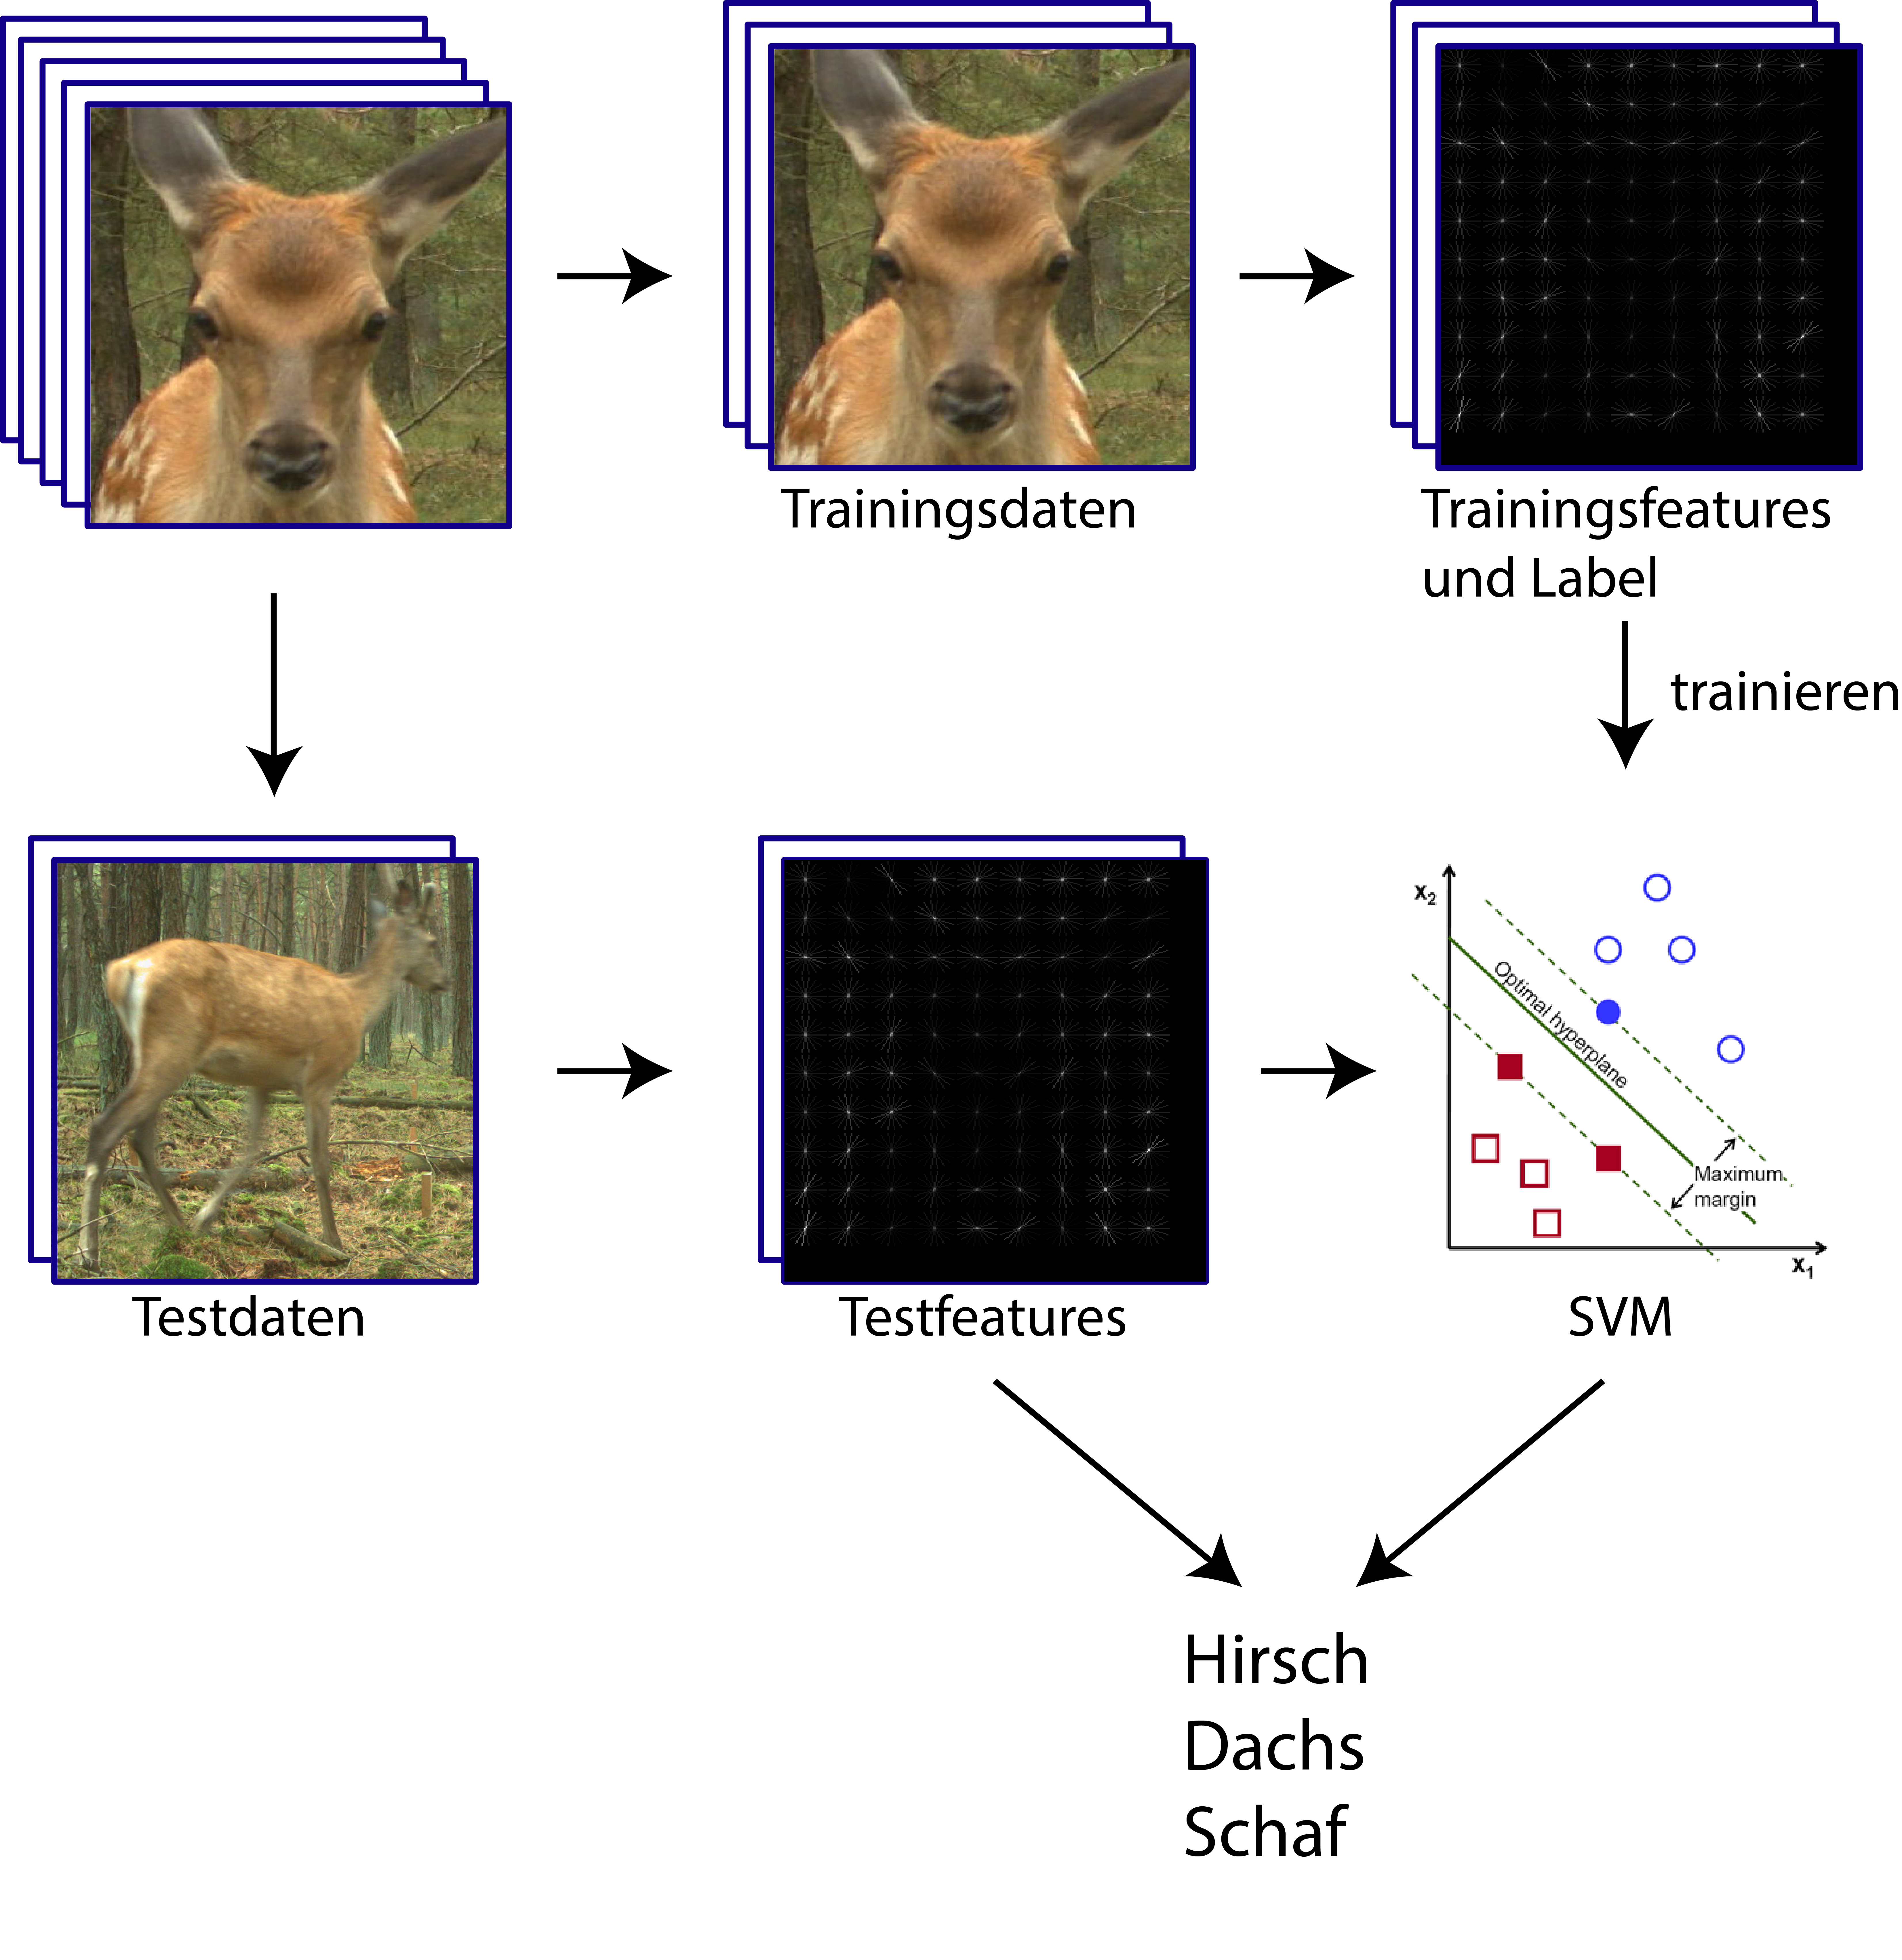
\includegraphics[scale=0.1]{img/ClassificationOverview.png}
		\caption{Übersichtsbild einer Klassifizierung}
	\end{figure}
\end{frame}

\begin{frame}[t,fragile]{Histogram of Oriented Gradients}
	\begin{figure}
		\centering
		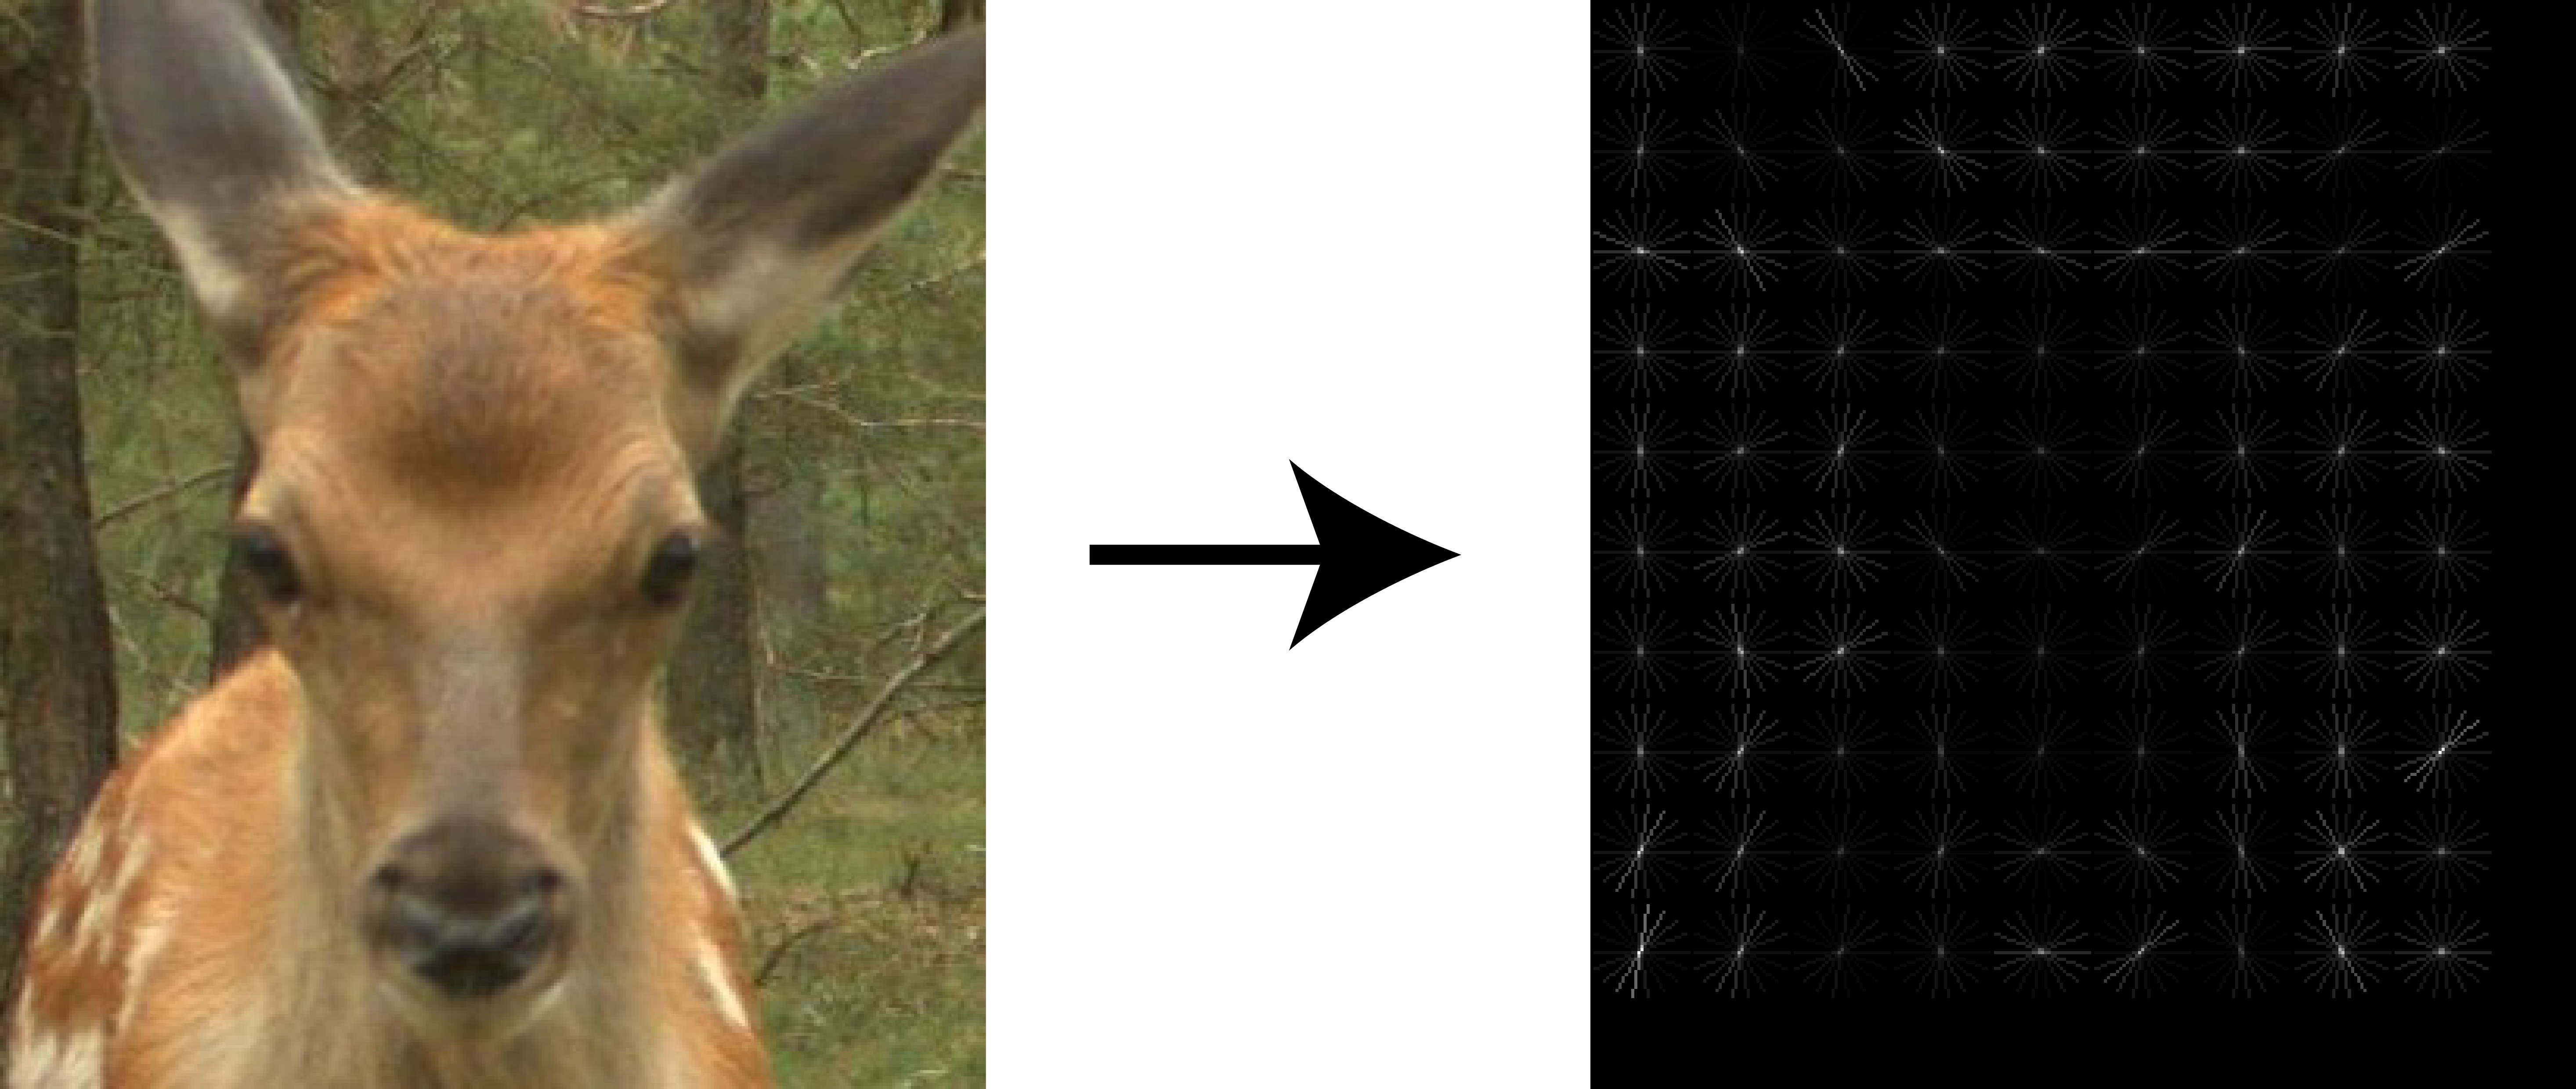
\includegraphics[scale=0.20]{img/Img2HOG.png}
		\caption{Visualisierung des HOG Feature Descriptors}
	\end{figure}
\end{frame}

\begin{frame}[t,fragile]{Berechnung des HOGs}
	\begin{enumerate}
 		\item Vorverarbeitung (optional)
		\item Gradienten Berechnung (Sobel)
	\begin{figure}
		\centering
		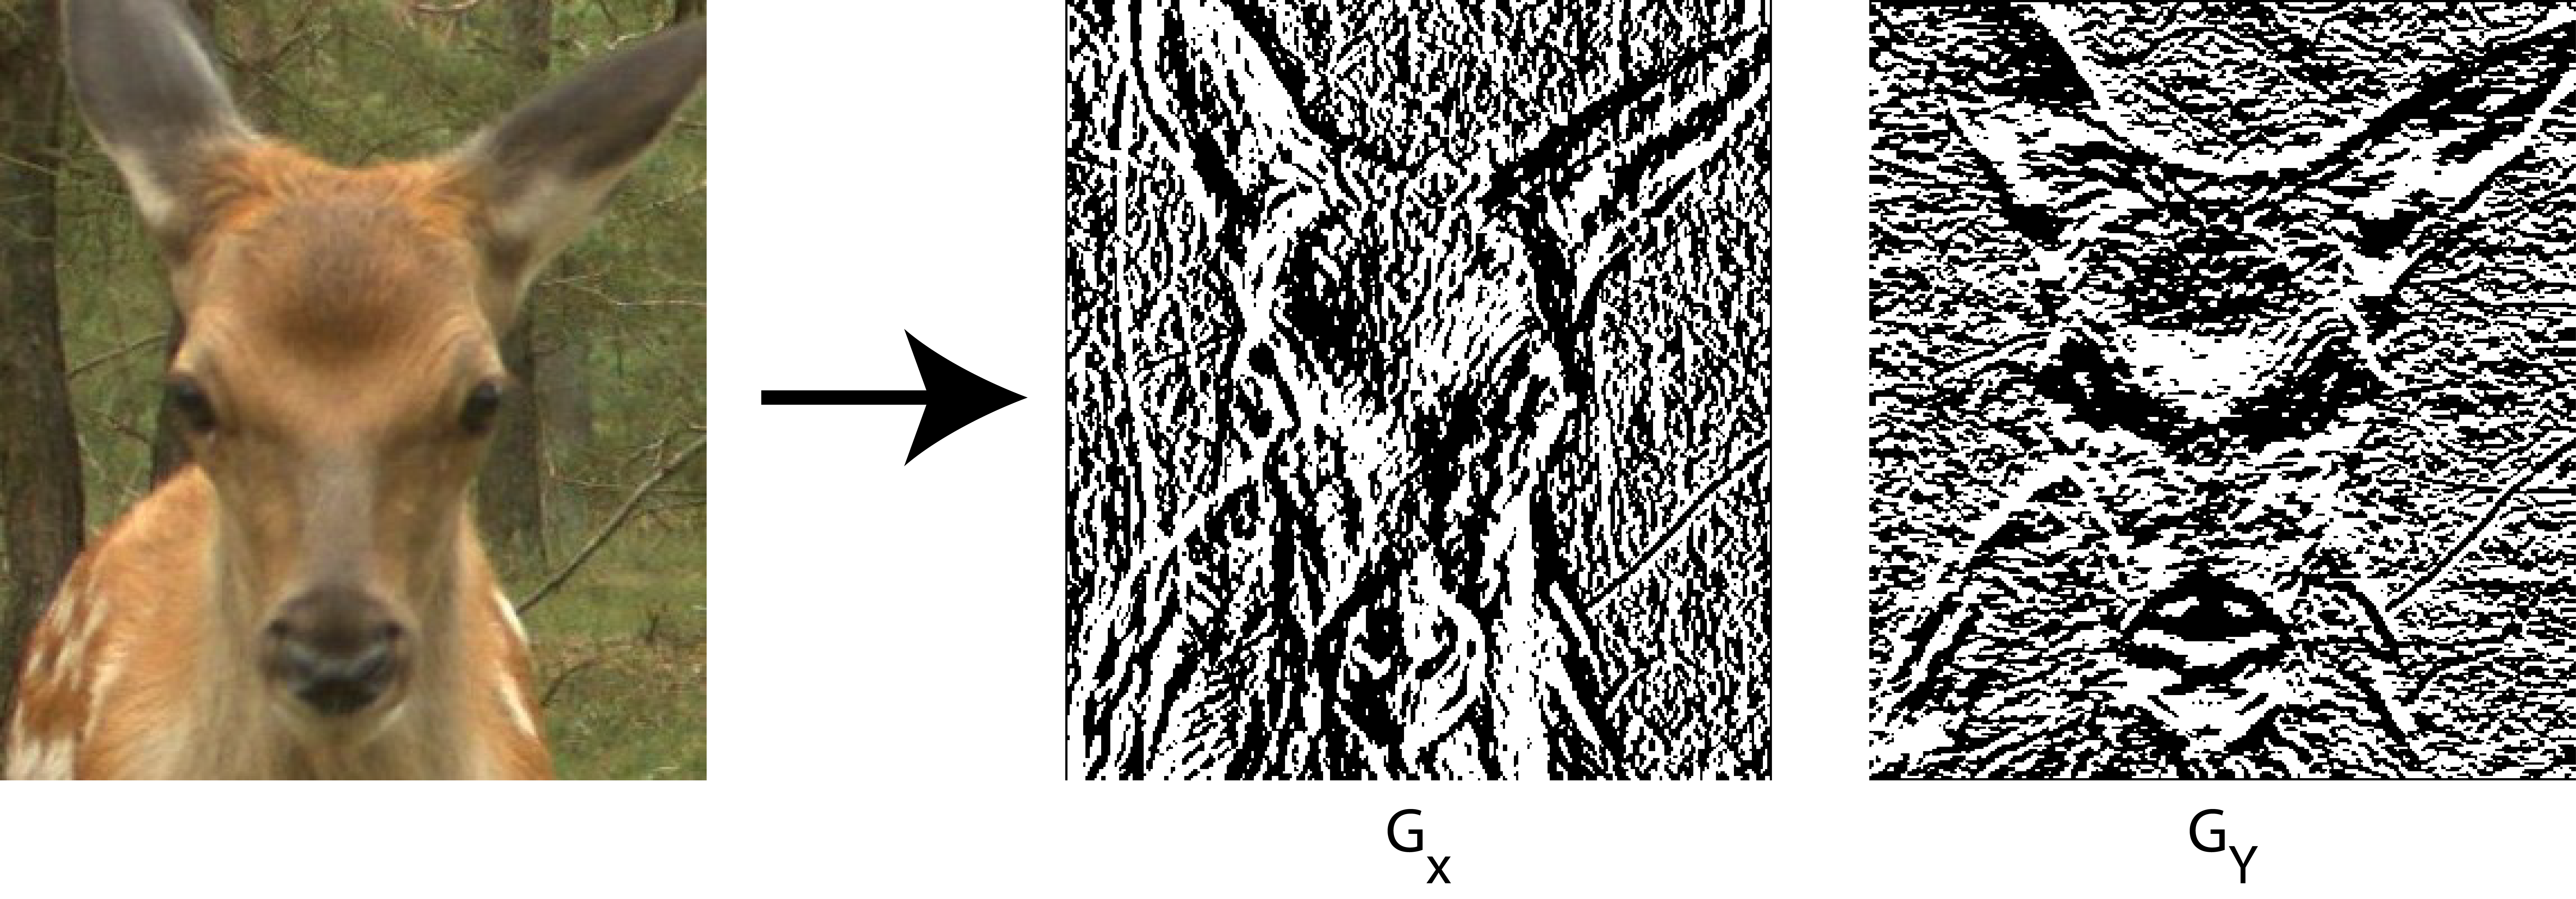
\includegraphics[scale=0.12]{img/sobel.png}
		\caption{Visualisierung der Gradientenberechnung }
	\end{figure}
  \end{enumerate}
	\begin{equation}
	Magnitude: |G| = \sqrt{G_x^2 + G_y^2}
	\end{equation}
\begin{equation}
    Orientierung: \Theta = \arctan({G_x, G_y})
\end{equation}
\end{frame}

\begin{frame}[t,fragile]{Berechnung des HOGs}
	\begin{enumerate}
 		\item Vorverarbeitung (optional)
		\item Gradienten Berechnung (Sobel)
		\item Unterteilung des Bildes in Rechtecke
		\item Extraktion eines Histogramms für jeden Block aus 4 Rechtecken
		\item Konkatenation der Histogramme zu einem gesamt Feature => HOGs
	\begin{figure}
		\centering
		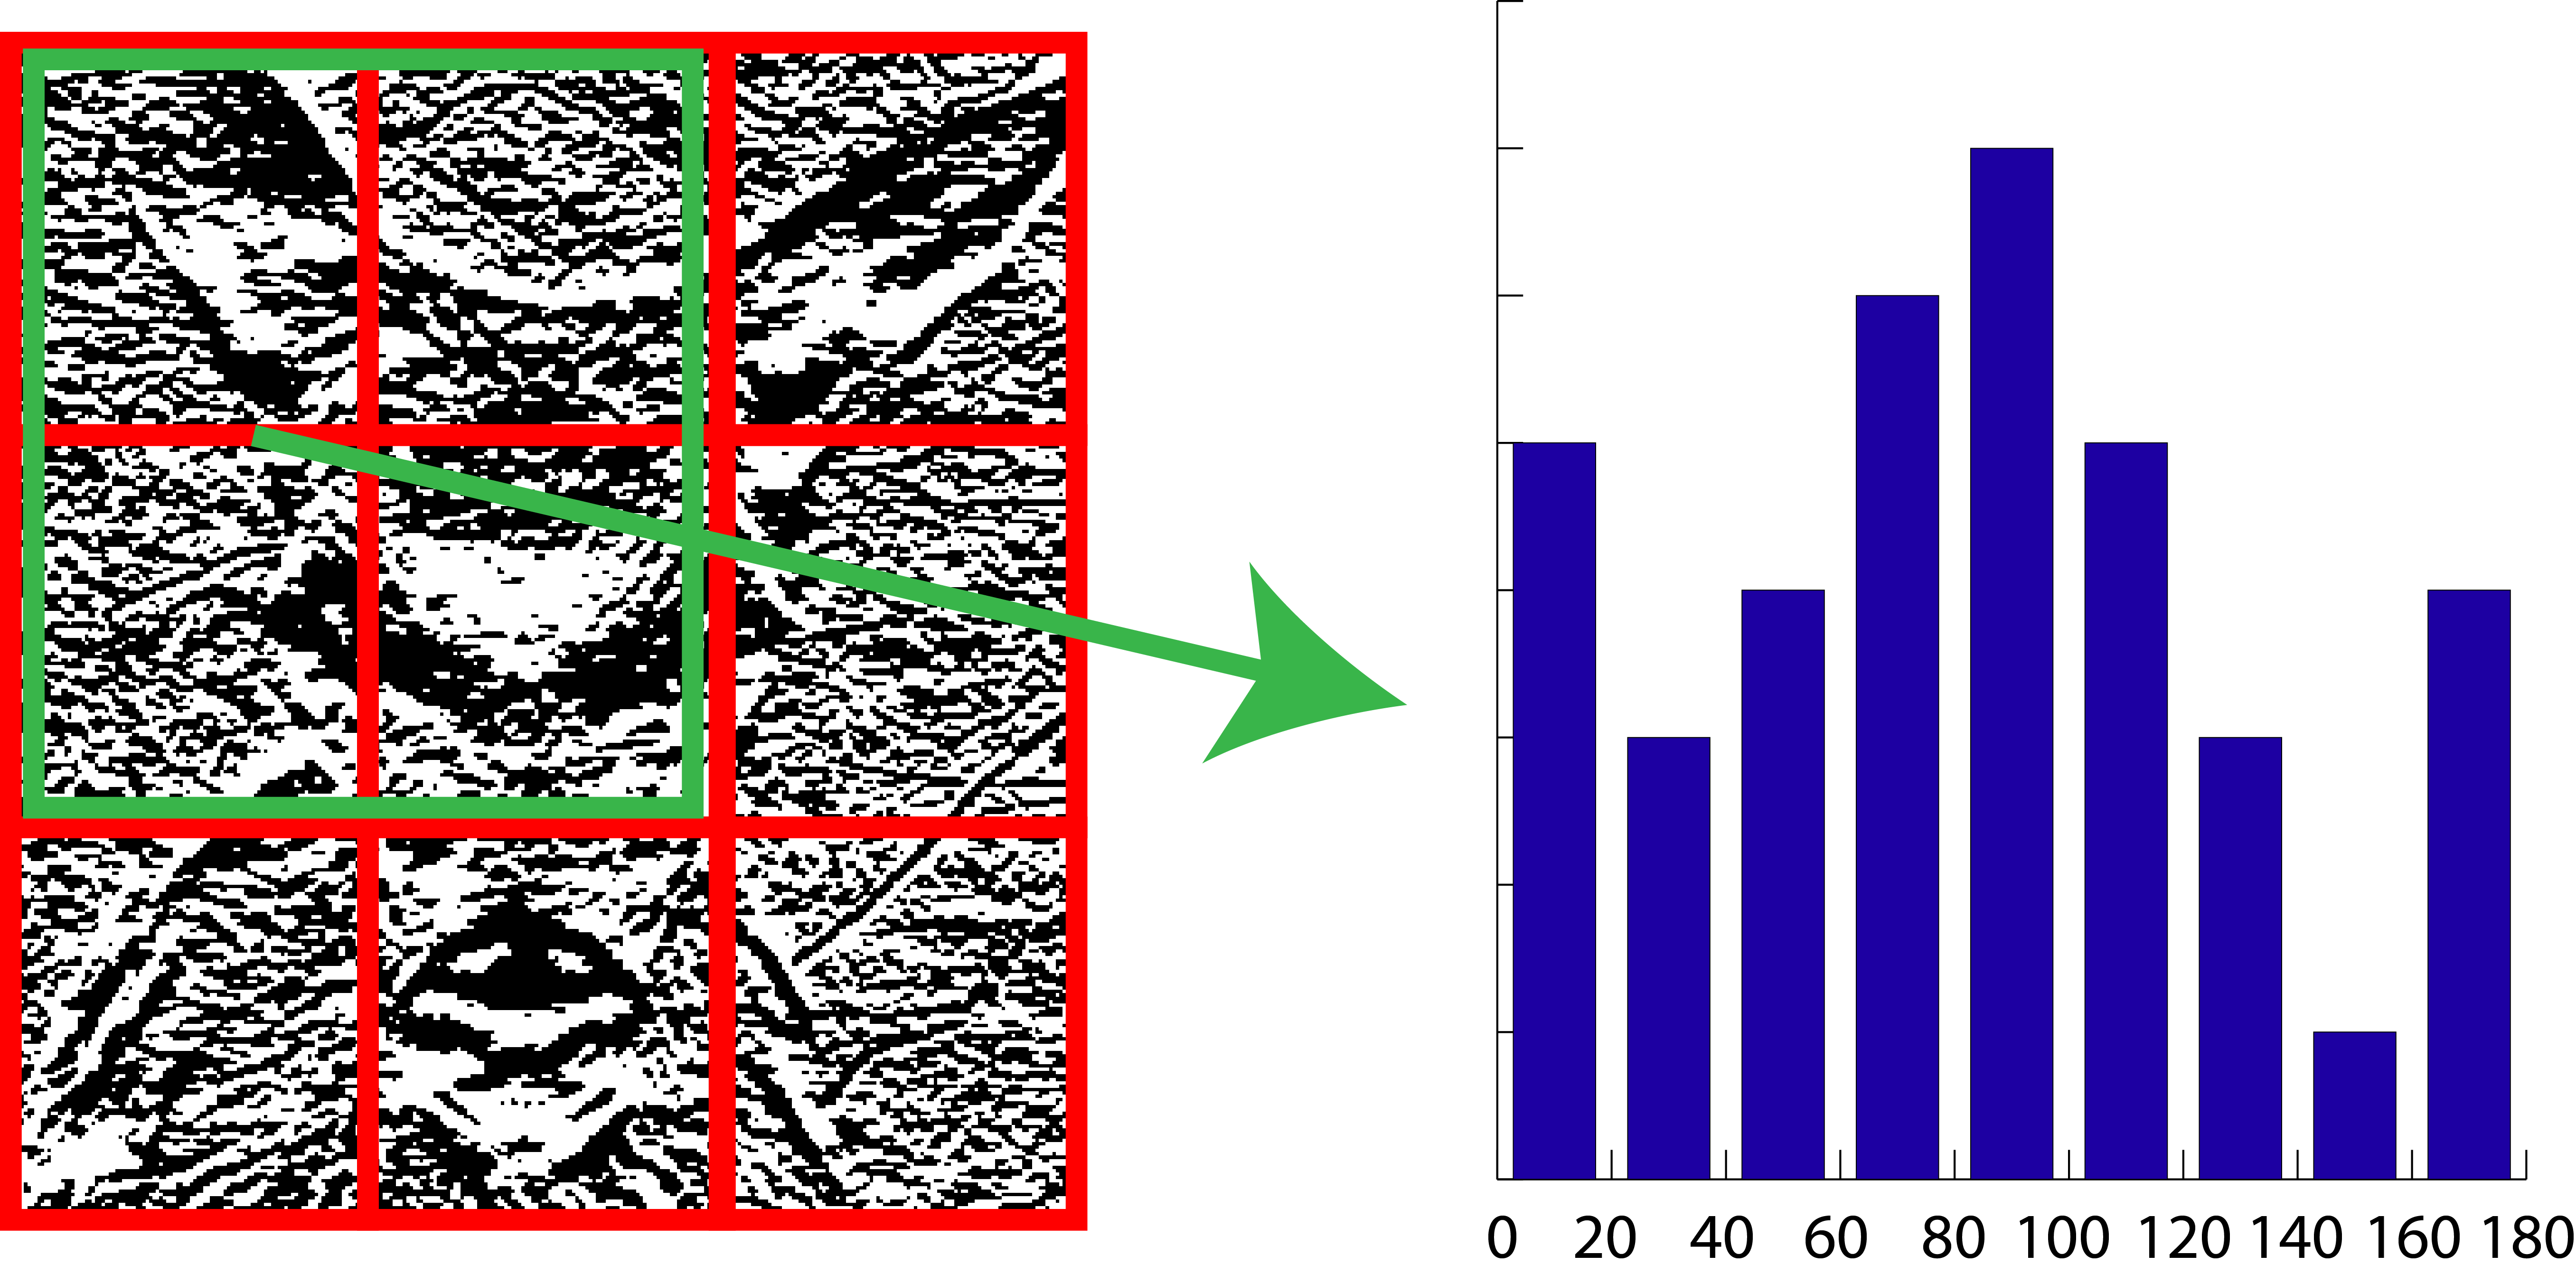
\includegraphics[scale=0.12]{img/sobel2hog.png}
		\caption{Berechnung eines Histogramms}
	\end{figure}	
  \end{enumerate}
\end{frame}

\begin{frame}[t,fragile]{Verwendete Support Vector Machine}
	\begin{itemize}
		\item openCV Implementierung
 		\item Kernel: Radiale Basisfunktion
		\item Bestrafung von Ausreißern
		\item Gewichtung eines Datenpunktes $\gamma = 0,5$
		\item $C = 12,5$
  	\end{itemize}
	\begin{figure}
		\centering
		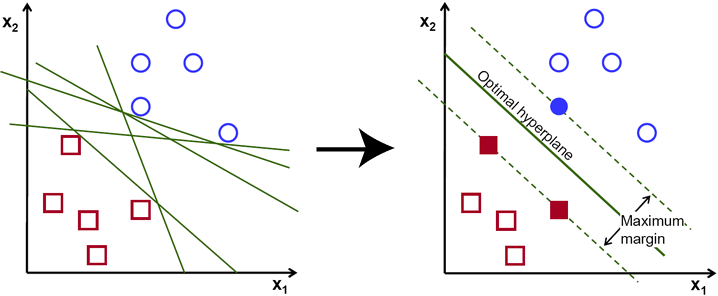
\includegraphics[scale=1]{img/SVM.png}
		\caption{Beispiel für eine Klassifizierung mit einer SVM (Quelle: \url{https://docs.opencv.org/3.4.2/d4/db1/tutorial_py_svm_basics.html)}}
	\end{figure}
\end{frame}

\begin{frame}[t,fragile]{Testparameter und Evaluierung}
  \begin{itemize}
 	\item Testparameter:
		\begin{itemize}
 			\item Dachs und Hirsch Tagesbilder
			\item Bis zu 66\% Trainingsdaten; Rest Testdaten
			\item Zusätzlich um gespiegelte Trainingsdaten erweitert

 		 \end{itemize}
  \end{itemize}
	\begin{table}
		\begin{tabular}{|c||c|c|c|c|}
			\hline
			Mittlere Präzision & standard & gespiegelt  \\
			\hline
			Hirsch & 96,3\% ($\sigma = 0.033$) & 94,5\% ($\sigma = 0.035$)  \\ 
			\hline
			Dachs & 81,3\% ($\sigma = 0.125$) & 83,7\% ($\sigma = 0.109$) \\
			\hline
		\end{tabular}
	\caption{Auswertung der durchschnittlichen Präzision des HOGs in Kombination mit einer SVM auf Testdaten mit zwei verschiedenen Labeln aus 50 Trainings- und Evaluierungs-Durchläufen. Die Parameter des HOG-Descriptors wurden zuvor optimiert. }
	\end{table}
  \begin{itemize}
 	\item Beobachtung: Eine Einheitliche Trainingsdatenmenge erhöht die Präzision deutlich
  \end{itemize}
\end{frame}


